%20130916 JW, first writing
\documentclass[iop]{emulateapj}


\usepackage{graphicx}
\usepackage{float}
\usepackage{amsmath,amsthm,amssymb}


\def\g{$g$}
\def\t{$t$}
\def\T{$T$}
\def\fillin{\#\#\#\#????}


\begin{document}


\title{Humpty Dumpty Had a Great Fall: Measuring the Acceleration due to Gravity with a Simple Pendulum}


\author{ Anthony Garcia
and
Joshua Wallace}
\affil{Advanced Undegrad Lab,Department of Physics and Astronomy, University of Utah,
 115 South 1400 East, Salt Lake City, UT 84112
}


\begin{abstract}


\g man, \g!


\end{abstract}


\section{Introduction}


Of the four fundamental forces of nature, gravity is the one that we have the 
most experience with in our everyday lives.  It is such a constant in our lives 
that every movement we make factors in the force of gravity, even if we are not
aware of it. We put objects down, expecting them to stay there because of 
gravity. A basketball player shoots a ball upwards, expecting the familiar 
parabolic arc due to gravity to bring it back down into the basket.  Even the
common phenomenon known as walking relies on gravity's pull to give our feet
the friction needed to push us forward. Our experience with gravity is so
intimate that we know exactly how things perform in earth's gravity field 
without having to measure and calculate (e.g. the basketball player knowing the 
right momentum to give the ball to score a basket without any calculation being
performed).


\g\ as a measure of force of gravity...


Importance of calculating g:  study mantle, earthquakes?, earth's density 
(similar to recent lunar probes), clock timing (which use pendula as well)...


To calculate \g, we will use a pendulum setup quite similar to that of the
pendulum clocks mentioned above.  Section~\ref{sec:theory} will introduce the 
physics behind this calculation more thoroughly.  Here we state the intended 
goals of our study of the motion of a simple pendulum:  (1) To be able to 
determine the value of \g, which as discussed above is an important parameter
for a variety of calculations; (2) to test a mathematical model (introduced in 
section~\ref{sec:theory}) of a physical system and compare the correspondence 
between the two and (3) use the process as an introduction into the sources of 
errors and their propagation to gain greater skills as a physicist-in-training. 
The experiment we will be performing is discussed in great detail in .......... 


\section{Theoretical Background}
\label{sec:theory}




Later gater...


Also talk about small angle approximation...


%%%%%%%%%%%%%%%%%%%%%%%%%%%%%%%%%%%%%%%%%%%%%%%%%%%%%%%%%%%%%%


\begin{figure}[H]
\centering
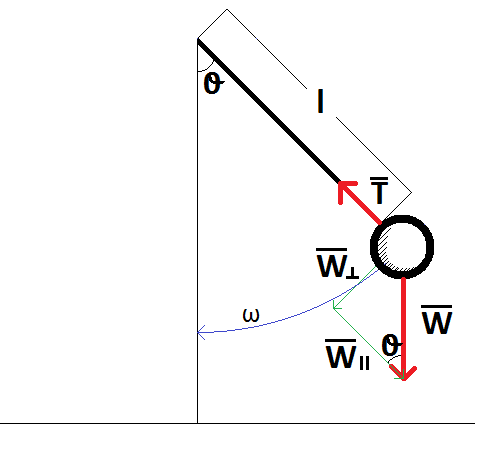
\includegraphics[width=85mm]{../../Images/FreebodyDiagram.png}
\caption{Diagram of a simple pendulum. The components listed are;
$\theta$ is the angle between the string
and the rest location of the pendulum, l is the length of the string,
$\vec{W}$ is the weight force of the bob (i.e. W = mg), $\vec{W}_\perp$ is the 
component of the weight force perpendicular to l, $\vec{W}_\parallel$ 
is the component of the weight force parallel to l.}
\label{Pendulum}
\end{figure}


The motion of a simple pendulum can be derived by analysing the torques (or forces) that acts 
on the bob of the pendulum. Assume the string that the pendulum hangs from is massless, and
its length l does not change. Friction on the string at the fulcrum as well as the
air drag on the bob is also ignored. See Appendix A for the full derivation
of the equation of motion for the simple harmonic oscillator.


From Figure 1; T is the tension force on the rope, l is the length of the
rope (or r$\cdot\hat{r}$, where $\hat{r}$ is a unit vector), $\theta$ is the angle, and W is the weight given by m$\cdot$g.


Using the small angle approximation
\begin{equation}
\boxed{sin\theta \approx \theta}
\end{equation}
for small angles, we derive the equation of motion
\begin{equation}
\boxed{T = 2\pi\sqrt{\frac{l}{g}}}
\end{equation}
to model a simple pendulum.
%%%%%%%%%%%%%%%%%%%%%%%%%%%%%%%%%%%%%%%%%%%%%%%%%%%%%%%%%%%%%%%


\section{Experimental Procedure}
\label{sec:procedure}


\subsection{Setup}


The setup consisted of a metal frame attached to a wall, a string, and a metal 
ball.


%%%%%%%%%%%%%%%%%%%%%%%%%%%%%%%%%%%%%%%%%%%%%%%%%%%%%%%%%%%%%%%%%


\begin{figure}[H]
\centering
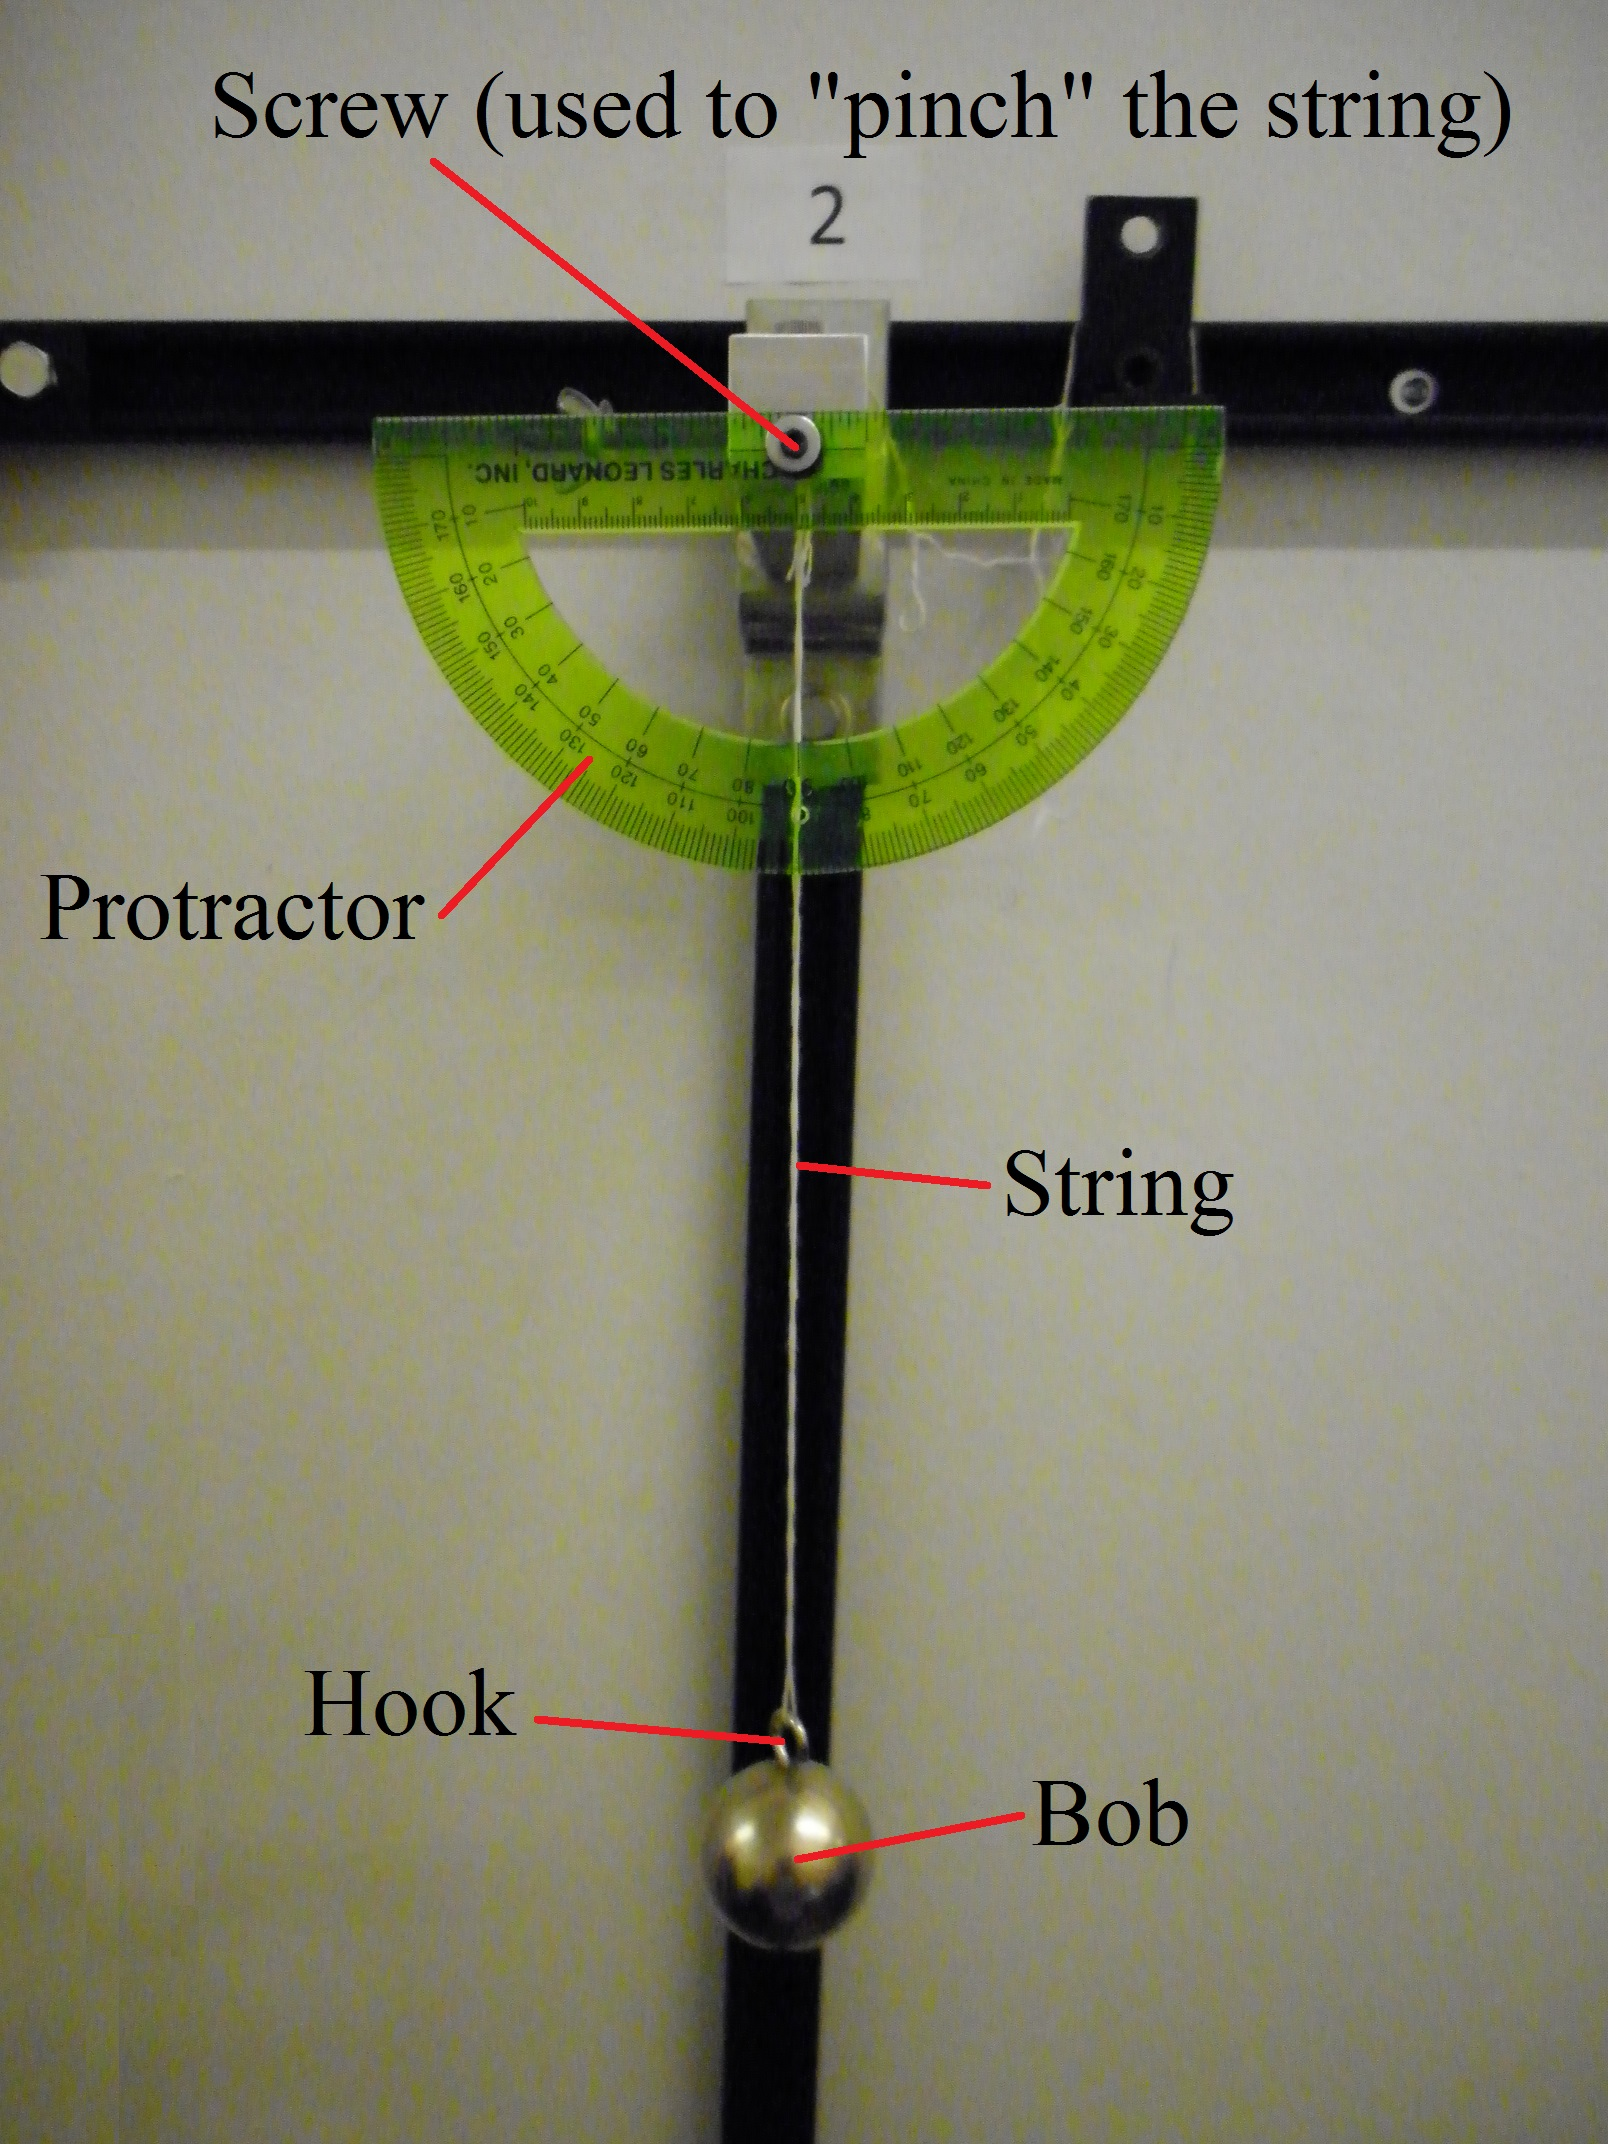
\includegraphics[width=85mm]{../../Images/Pendulum.JPG}
\caption{The bob is hung from the string by its hook. A screw pinches the string to act as
the pendulum's fulcrum. We measured the angle of the initial period with the 
protractor.}
\label{Pendulum}
\end{figure}


%%%%%%%%%%%%%%%%%%%%%%%%%%%%%%%%%%%%%%%%%%%%%%%%%%%%%%%%%%%%%%%%%%


\subsection{Procedure}


The first measurements we made were those of the ball diameter and the length 
of the hook on the top of the ball.  These data are contained in table \#\#\#\#\#. 
These measurements were made using ???\#\#\#a vernier caliper.  Due to the size of 
the ball and the large uncertainty associated with measuring the full length 
from the pivot point to the ball center (the center of mass of the
ball) we decided it would be best to measure the length of the string from the
pivot point to the top of the hook of the ball and then add the measured values 
for the hook height and ball radius afterwards.  The uncertainties from the 
caliper measurements are small enough compared to the uncertainty in using 
either a measuring stick or a tape measure in determining the length of the
string that making three separate measurements like this do not create an 
unnecessarily large uncertainty in length.  As stated above, a tape measure 
and/or measuring stick were used to measure the distance from the pivot point
to the top of the hook.  This was the distance that was measured when the
pendulum length was varied.


The next step was to determine the uncertainty of the stopwatch we used.  The
stopwatches we used were brand \#\#\#\#\#.  There were two sources of systematic 
uncertainty in the time measurements made by the stopwatch.  The first was the 
gain/lag the stopwatch had over real time.  The second was simply the finite 
gradations of time measured by the stopwatch ($.01 s$).  To account for the 
first source of systematic error (and also to determine which of the two 
authors were most accurate and precise in their time measurements) we timed 
ourselves against an atomic clock for 1s and 100s intervals.  (On the second
day, 20s and 50s intervals).  These data are available in table \fillin.  JW 
was determined to have the best combination of accuracy and precision and was 
designated as the official timekeeper for the duration of the study.  As seen 
in table \fillin, the mean of the time measurements were not equal to the time 
interval attempted to be measured.  This gain/lag were accounted for in our 
final results by finding an appropriate ``weighting factor'' by which to 
multiply all our time measurements to increase their accuracy.  The weighting 
factor was calculated as follows:


\begin{equation}
\label{eq:timeweight}
W = 1 + \frac{t_{atomic}-t_{mean}}{t_{atomic}} 
\end{equation}


where $t_{atomic}$ is the real time as measured by the atomic clock 
and $t_{mean}$ is the mean of the times measured by the 
stopwatch.  The fraction determines what percent of the real time was measured 
by the average of the stopwatch times, which is then added to $1$ to provide a 
multiplicative factor to correct our time measurements.  The standard deviation 
of the measured times is included in our final calculation of the error of $T$. 


Measuring against the atomic clock provided a measure of both the stopwatch's 
own limitations and the user's reaction time.  However, it is impossible to 
separate the two.  In order to fully account for the user's reaction time the 
above error was assumed to be due entirely to the stopwatch's limitations and 
a separate calculation was made of the timekeeper's reaction time.  The 
timekeeper recorded himself pushing the start and stop button on the stopwatch 
as fast as possible.  The data from this exercise are recorded in table \fillin. 
The average was $.17s$; this number was added to the overall uncertainty of $T$. 


The next thing we did was determine the best way to measure the period of the 
pendulum's swing, i.e., a method that would allow us to both be accurate 
(allowing us to obtain a true value for \g) and precise (thus reducing random 
error). We first compared whether it was better to start timing a period from 
when the ball was released or to wait a period and start timing with the 
second period.  We wanted to see if there was a difference in accuracy and 
precision between the simultaneous double hand movement of releasing the ball 
while starting the stopwatch and just timing the period by eye. For this we 
timed a single swing of the pendulum eight times for both cases (i.e. starting 
timing with the swing and starting timing with the second swing) this was done 
for two different lengths: one around $26cm$ and the other around \fillin$cm$. 
These data are shown in table \fillin. Unfortunately the method with the lowest 
mean (timing from release) had the largest spread in times measured and 
vice-versa (for timing the second period). We chose to go 
with the method with the least uncertainty (i.e. lowest spread, or timing the 
second swing) over greatest accuracy because we figured that the method we 
used to determine the stopwatch gain/lag was closest to the method that timed 
the second swing; for both methods, the start and stop time were determined by 
eye.  If we had pushed a button on the atomic clock to start its timing at the 
same moment we had started the stopwatch, then this method would have been 
more similar to the method that used the release time of the pendulum to 
measure \T.  Therefore, the weighting factor determined by the timing against 
the atomic clock method factors in the inaccuracy of the second method more 
than the first method (in addition to the stopwatch's own gain/lag). The 
inaccuracy of the second method being thus accounted for we are free to choose 












\section{Data and Results}
\label{sec:data}


%%%%%%%%%%%%%%%%%%%%%%%%%%%%%%%%%%%%%%%%%%%%%%%%%%%%%%%%%%%%%%%%


\begin{table}[H]
\caption{Atomic Clock Measurements} % title of Table
\centering % used for centering table
\begin{tabular}{c c} % centered columns (4 columns)
\hline\hline %inserts double horizontal lines
Time Lapse & Stop Watch Time (s) \\ [0.5ex] % inserts table
%heading
\hline % inserts single horizontal line
50s & 49.85 \\ % inserting body of the table
    & 49.99 \\
    & 50.05 \\
    & 50.09 \\
    & 49.98 \\
$\overline{At}$ & 49.99 \\
$\sigma_{\overline{At}}$ & 0.04 \\    [1ex] % [1ex] adds vertical space
\hline %inserts single line
\end{tabular}
\label{table:nonlin} % is used to refer this table in the text
\end{table}


\begin{table}[H]
\caption{Reaction Time} % title of Table
\centering % used for centering table
\begin{tabular}{c c} % centered columns (4 columns)
\hline\hline %inserts double horizontal lines
& Stop Watch Reaction Time (s) \\ [0.5ex] % inserts table
%heading
\hline % inserts single horizontal line
& 0.15 \\ % inserting body of the table
& 0.13\\
& 0.15\\
& 0.14\\
& 0.17\\
$\overline{Rt}$ & 0.15 \\
$\sigma_{\overline{Rt}}$ & 0.01 \\    [1ex] % [1ex] adds vertical space
\hline %inserts single line
\end{tabular}
\label{table:nonlin} % is used to refer this table in the text
\end{table}




\begin{table}[H]
\caption{Period Measurement for Varying Lengths} %title of the table
\centering % centering table
\begin{tabular}{c rrrrr c} % creating eight columns
\hline\hline %inserting double-line
Length (m) & \multicolumn{5}{c}{$T_{20}$ (s)} & $\overline{T^2}$ ($s^2$)\\ [0.5ex]
\hline % inserts single-line
0.280 & 22.68 & 22.64 & 22.64 & 22.58 & 22.56 & 6.19\\ % Entering row contents
0.415 & 27.03 & 27.05 & 27.07 & 27.03 & 27.06 & 5.78\\
0.546 & 30.61 & 30.74 & 30.57 & 30.65 & 30.58 & 5.37\\
0.638 & 32.97 & 33.04 & 33.05 & 33.03 & 32.96 & 4.75\\
0.800 & 36.70 & 36.65 & 36.73 & 36.74 & 36.71 & 4.13\\
0.989 & 40.65 & 40.73 & 40.62 & 40.62 & 40.72 & 3.37\\
1.143 & 43.60 & 43.61 & 43.59 & 43.56 & 43.53 & 2.72\\
1.293 & 46.33 & 46.46 & 46.40 & 46.26 & 46.29 & 2.34\\
1.395 & 48.01 & 48.06 & 48.12 & 48.17 & 48.09 & 1.83\\
1.498 & 49.77 & 49.82 & 49.81 & 49.72 & 49.70 & 1.28\\ [1ex] % [1ex] adds vertical space
\hline % inserts single-line
\end{tabular}
\label{tab:hresult}
\end{table}


\begin{table}[H]
\caption{Dimensions of the bob} %title of the table
\centering % centering table
\begin{tabular}{c c c} % creating eight columns
\hline\hline %inserting double-line
Quantity & Uncertainty in Measurment & Measured Value\\ [0.5ex]
\hline % inserts single-line
Mass (g) & $\pm$ 0.1 & 226.2\\ % Entering row contents
Diameter (mm) & $\pm$ 0.03 & 38.02\\
Radius (m) & $\pm$ 0.00002 & 0.01901\\
Hook Length (mm)& $\pm$ 0.03 & 11.95\\
Hook Length (m)& $\pm$ 0.00003 & 0.01195\\[1ex] % [1ex] adds vertical space
\hline % inserts single-line
\end{tabular}
\label{tab:hresult}
\end{table}


%%%%%%%%%%%%%%%%%%%%%%%%%%%%%%%%%%%%%%%%%%%%%%%%%%%%%%%%%%%%%%%%%


















\section{Discussion}
\label{sec:discuss}
































\section{Conclusion}






%%%%%%%%%%%%%%%%%%%%%%%%%%%%%%%%%%%%%%%%%%%%%%%%%%%%%%%


\appendix
\numberwithin{equation}{section}
\section{Appendix A: Deriving the Equation of Motion for the Simple Pendulum}


The motion of a simple pendulum can be derived by analysing the torques (or forces) that acts 
on the bob of the pendulum. Assume the string that the pendulum hangs from is massless, and
its length l does not change. Friction on the string at the fulcrum as well as the
air drag on the bob is also ignored. The definition of torque is given by;
\begin{equation}
\boxed{\tau = \vec{r} \times \vec{F} \equiv |\vec{r}||\vec{F}|\hat{n}sin\theta}
\end{equation}
From Figure 1; T is the tension force on the rope, l is the length of the
rope (or r$\cdot\hat{r}$, where $\hat{r}$ is a unit vector), $\theta$ is the angle, and W is the weight given by m$\cdot$g.
Using the definition of the cross product;
\begin{align*}
\tau_T & = \vec{l} \times \vec{T} = 0 & \text{($\vec{l}$ is $||$ to $\vec{T}$)}\\
\tau_W & = \vec{l} \times \vec{W}\\
& = |\vec{l}||\vec{W}|\hat{n}sin\theta\\
& = -l\cdot W\cdot sin\theta & \text{($\hat{n}$ is "-")}\\
& = -l\cdot mg\cdot sin\theta & \text{(W = m$\cdot$g)}\\
\end{align*}
\begin{equation}
\boxed{\tau_W = -lmgsin\theta}
\end{equation}
Newton's second law applied to rotational motion is given by,
\begin{equation}
\tau = I\cdot\alpha
\end{equation}
where I is the moment of inertia. The simple pendulum will be 
treated as a point particle at a distance l from the origin.
Equating the two we get;
\begin{align*}
\tau_W = -lmgsin\theta & = I\cdot\alpha\\
& = (ml^2)\alpha & \text{(I = $ml^2$ for a point particle)}\\
& = (ml^2)\ddot{\theta} & \text{($\alpha = \ddot{\theta}$)}\\
\Rightarrow -gsin\theta & = l\ddot{\theta}\\
\Rightarrow l\ddot{\theta} + gsin\theta & = 0
\end{align*}
The Taylor series of sin($\theta$) is given by
\begin{equation}
\boxed{sin\theta = \theta - \frac{\theta^3}{3!} + \frac{\theta^5}{5!} - \frac{\theta^7}{7!} + \frac{\theta^9}{9!} - ...}
\end{equation}
For small angles we get
\begin{equation}
\boxed{sin\theta \approx \theta}
\end{equation}
which is the small angle approximation. Note that the small angle approximation 
is valid to about $15^{\circ}$.\\
Applying the small angle approximation to our equation of motion we get
\begin{align}
\boxed{l\ddot{\theta} + g\theta = 0}
\end{align}
Solving the the differential equation;
\begin{align*}
l\ddot{\theta} + g\theta & = 0\\
\Rightarrow \ddot{\theta} + \frac{g}{l}\theta & = 0\\
\end{align*}
The characteristic equation for this Differential Equation is
\begin{align*}
x^2 + \frac{g}{l} = 0\\
\Rightarrow x = \pm i\sqrt{\frac{g}{l}}
\end{align*}
Which has the general equation
\begin{align*}
\theta(t) & = C_1e^{i\sqrt{(g/l)}t} + C_2e^{-i\sqrt{(g/l)}t}\\
& = C_1[cos(\sqrt\frac{g}{l}t) + isin(\sqrt\frac{g}{l}t)] +\\ 
&~~~~~~+ C_2[cos(\sqrt\frac{g}{l}t) - isin(\sqrt\frac{g}{l}t)]\\
& = (C_1 + C_2)cos(\sqrt\frac{g}{l}t) + i(C_1 - C_2)sin(\sqrt\frac{g}{l}t)\\
& = Acos(\sqrt\frac{g}{l}t) + Bsin(\sqrt\frac{g}{l}t)\\
\end{align*}
If we create a right triangle with the constants A and B, to get a hypotenuse
constant C and angle $\phi$. That triangle can be describe with the terms;
\begin{align*}
sin\phi & = \frac{B}{C}\\
cos\phi & = \frac{A}{C}
\end{align*}
Then if we multiply the general solution by C/C;
\begin{align*}
\theta(t) & = C[\frac{A}{C}cos(\sqrt\frac{g}{l}t) + \frac{B}{C}sin(\sqrt\frac{g}{l}t)]\\
& = C[cos(\phi) cos(\sqrt\frac{g}{l}t) + sin(\phi)cos(\sqrt\frac{g}{l}t)]\\
& = C[cos(\phi) cos(\sqrt\frac{g}{l}t) - sin(-\phi)cos(\sqrt\frac{g}{l}t)]\\
& = C[cos(\sqrt\frac{g}{l}t - \phi)]
\end{align*}
$\phi$ is the phase shift. For the simple pendulum the phase shift is zero 
because the initial angle is $\theta_0$. This gives\\
\begin{equation*}
\theta(t) = Ccos(\sqrt\frac{g}{l}t)
\end{equation*}
Then for t = 0
\begin{align*}
\theta(0) & = C[cos(0)]\\
& = C\\
& \equiv \theta_0
\end{align*}
Then the solution to the equation of motion is
\begin{equation}
\boxed{\theta(t) = \theta_0[cos(\sqrt\frac{g}{l}t)]}
\end{equation}
We know that the derivative of $\theta(t)$ is $\omega$ (angular velocity)
\begin{align*}
\dot{\theta}(t) & = \omega(t)\\
& = -\sqrt\frac{g}{l}\theta_0[sin(\sqrt\frac{g}{l}t)]
\end{align*}
Angular velocity is zero every time it reaches the max height during an oscillation. We can than see for
for what times this occurs by setting $\omega \equiv 0$.
\begin{align*}
\omega & \equiv 0\\
-\sqrt\frac{g}{l}\theta_0[sin(\sqrt\frac{g}{l}t_n)] & = 0\\
\Rightarrow \sqrt\frac{g}{l}t_n & = sin^{-1}(0)\\
& = 2\pi n\\
\Rightarrow t_n & = 2\pi n\sqrt\frac{l}{g}
\end{align*}
This periodicity is what we call the Period;
\begin{equation}
\boxed{T = 2\pi \sqrt\frac{l}{g}}
\end{equation}
%%%%%%%%%%%%%%%%%%%%%%%%%%%%%%%%%%%%%%%%%%%%%%%%%%%%%%%%%










\acknowledgments


We thank ....










\begin{thebibliography}{}


%\bibitem[


\end{thebibliography}{}


\end{document}

